\chapter{Lab and place}
\section{The MIVIA Laboratory}

\begin{wrapfigure}[2]{l}{2cm}
	\vspace{-7mm}
	
\includegraphics[width=2cm]{images_not_compressed/MIVIALogo.jpg}
	\end{wrapfigure}
 for Macchine Intelligenti per il riconoscimento di Video, Immagini e Media which means intelligent machines for video, images and media recognition. The laboratory is located in Fisciano, Campania, Italy, near Salerno and Napoli as we can see in the figure \ref{location}.
 \begin{figure}[h]
 \begin{center}
	 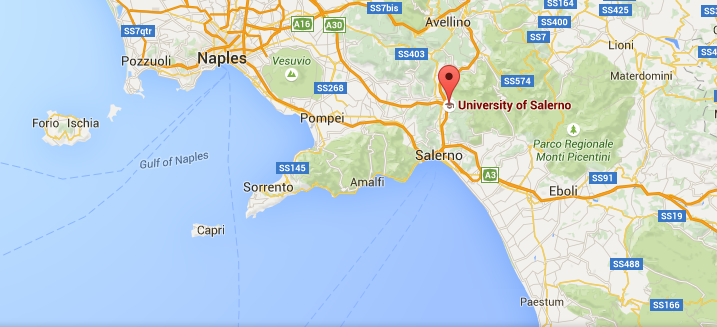
\includegraphics[width=15cm]{images_not_compressed/geoUniversity.png}
		\caption{Location of the University}
		\label{location}
	 \end{center}
 \end{figure}
 \par Besides teaching computer sciences, doctors of the lab work on pattern recognition, classification, media analysis and many parallel subjects like autonomous drones and robot vision.
 \par The laboratory is directed by Mario Vento. He is assisted by Alessia Saggese. Pasquale Foggia, Gennaro Percannella and Pierluigi Ritrovato (who is also my tutor). They are all teachers and researchers in the lab. There are also several students and graduated that work on thesis in the laboratory. I was more in contact with Antonio Greco and Raffaele Iuliano. All students and graduated was working on different projects and startups and the laboratory itself works for and with international companies.
 \par You can find all of this information on their website at this address : \url{http://mivia.unisa.it/}
 \par Because of the opportunity of double diploma, the proximity to France, the possibility to learn a new language even if we spoke English between us, I was really optimistic about the place and the laboratory.
